Over the past years, the integration of NFV with other technologies, such as SDN, Cloud
computing, and 5G \cite{5} has attracted significant attention from both the academic research
community and industry.
NFV integration with SDN and Cloud computing is beneficial due to the complementary
features and distinctive approaches followed by each technology toward providing solutions
to today?s and future networks \cite{6}, \cite{7}. For instance, NFV provides function abstraction
(i.e., virtualization of network functions) supported by ETSI \cite{8}, SDN provides network
abstraction supported by Open Networking Foundation (ONF) \cite{9}, and Cloud computing
provides computation abstraction (i.e., a shared pool of configurable computing resources
(e.g., networks, servers, storage, applications, and services)) supported by the Distributed
Management Task Force (DMTF) \cite{10}. Abstraction is one of the core features of cloud
computing which allows abstraction of the physical implementation to hide the background
(technical) details from users and developers. To summarize the relationships between NFV,
SDN, and Cloud computing, we use Figure 3.
\begin{figure}[h]
    \centering
    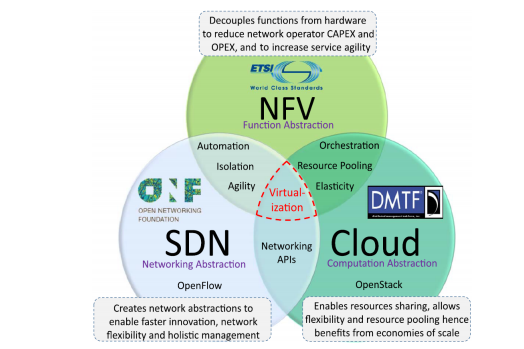
\includegraphics[width=1\textwidth]{2_2_4_integration}
    \caption{ETSI NFV reference architecture}
    \label{fig:2_2_4_integration}
\end{figure}
SDN, NFV, and Cloud computing technologies are complementary to each other but are
independent and can be deployed alone or together. A combination of these technologies together in a network architecture is more desirable \cite{11}. In fact, the advantages that accrue
from each of them are similar: agility, cost reduction, dynamism, automation, resource
scaling, etc.